% Options for packages loaded elsewhere
\PassOptionsToPackage{unicode}{hyperref}
\PassOptionsToPackage{hyphens}{url}
%
\documentclass[
]{article}
\usepackage{lmodern}
\usepackage{amssymb,amsmath}
\usepackage{ifxetex,ifluatex}
\ifnum 0\ifxetex 1\fi\ifluatex 1\fi=0 % if pdftex
  \usepackage[T1]{fontenc}
  \usepackage[utf8]{inputenc}
  \usepackage{textcomp} % provide euro and other symbols
\else % if luatex or xetex
  \usepackage{unicode-math}
  \defaultfontfeatures{Scale=MatchLowercase}
  \defaultfontfeatures[\rmfamily]{Ligatures=TeX,Scale=1}
\fi
% Use upquote if available, for straight quotes in verbatim environments
\IfFileExists{upquote.sty}{\usepackage{upquote}}{}
\IfFileExists{microtype.sty}{% use microtype if available
  \usepackage[]{microtype}
  \UseMicrotypeSet[protrusion]{basicmath} % disable protrusion for tt fonts
}{}
\makeatletter
\@ifundefined{KOMAClassName}{% if non-KOMA class
  \IfFileExists{parskip.sty}{%
    \usepackage{parskip}
  }{% else
    \setlength{\parindent}{0pt}
    \setlength{\parskip}{6pt plus 2pt minus 1pt}}
}{% if KOMA class
  \KOMAoptions{parskip=half}}
\makeatother
\usepackage{xcolor}
\IfFileExists{xurl.sty}{\usepackage{xurl}}{} % add URL line breaks if available
\IfFileExists{bookmark.sty}{\usepackage{bookmark}}{\usepackage{hyperref}}
\hypersetup{
  pdftitle={Using Tikz},
  pdfauthor={Dan Li},
  hidelinks,
  pdfcreator={LaTeX via pandoc}}
\urlstyle{same} % disable monospaced font for URLs
\usepackage[margin=1in]{geometry}
\usepackage{graphicx}
\makeatletter
\def\maxwidth{\ifdim\Gin@nat@width>\linewidth\linewidth\else\Gin@nat@width\fi}
\def\maxheight{\ifdim\Gin@nat@height>\textheight\textheight\else\Gin@nat@height\fi}
\makeatother
% Scale images if necessary, so that they will not overflow the page
% margins by default, and it is still possible to overwrite the defaults
% using explicit options in \includegraphics[width, height, ...]{}
\setkeys{Gin}{width=\maxwidth,height=\maxheight,keepaspectratio}
% Set default figure placement to htbp
\makeatletter
\def\fps@figure{htbp}
\makeatother
\setlength{\emergencystretch}{3em} % prevent overfull lines
\providecommand{\tightlist}{%
  \setlength{\itemsep}{0pt}\setlength{\parskip}{0pt}}
\setcounter{secnumdepth}{-\maxdimen} % remove section numbering
\usepackage{tikz}
\usepackage{pgfplots}

\title{Using Tikz}
\author{Dan Li}
\date{2020-08-14}

\begin{document}
\maketitle

\hypertarget{tikz-picture}{%
\subsection{TikZ picture}\label{tikz-picture}}

\begin{itemize}
\tightlist
\item
  Here is a TikZ picutre
\end{itemize}

\textbackslash begin\{tikzpicture\} \textbackslash draw (0,0) circle
(2cm); \textbackslash end\{tikzpicture\}

\begin{tikzpicture}
\draw (0,0) circle (2cm);
\end{tikzpicture}

\begin{itemize}
\tightlist
\item
  Here is another TikZ picutre
\end{itemize}

\textbackslash begin\{tikzpicture\}
\textbackslash begin\{axis\}{[}xmax=9,ymax=9, samples=50{]}
\textbackslash addplot{[}blue, ultra thick{]} (x,x\emph{x);
\textbackslash addplot{[}red, ultra thick{]} (x}x,x);
\textbackslash end\{axis\} \textbackslash end\{tikzpicture\}

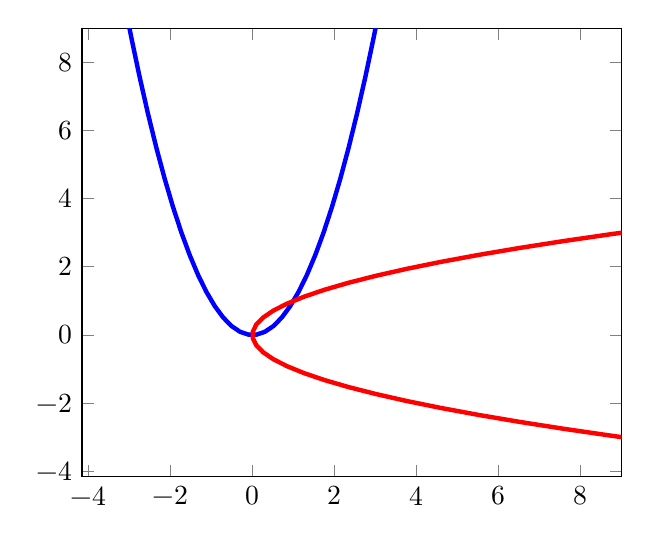
\begin{tikzpicture}
\begin{axis}[xmax=9,ymax=9, samples=50]
  \addplot[blue, ultra thick] (x,x*x);
  \addplot[red,  ultra thick] (x*x,x);
\end{axis}
\end{tikzpicture}

\end{document}
